\begin{figure}[p]
\centering
\captionsetup{justification=raggedright,labelsep=none,singlelinecheck=false,labelformat=boldlabel}
\caption[]{\footnotesize \textbf{: Sequential changes in out-of-sample RMSE relative to HAR.} Each column considers one extension of HARX. The bars first add exogenous covariates, then the indicated model extension, and finally the equal-weighted forecast combination. Positive changes represent lower RMSE. These arithmetic comparisons do not identify causal contributions.}
\label{fig:rv-sequential_waterfall}
\par\smallskip\textbf{Panel A. Long sample}\par\smallskip
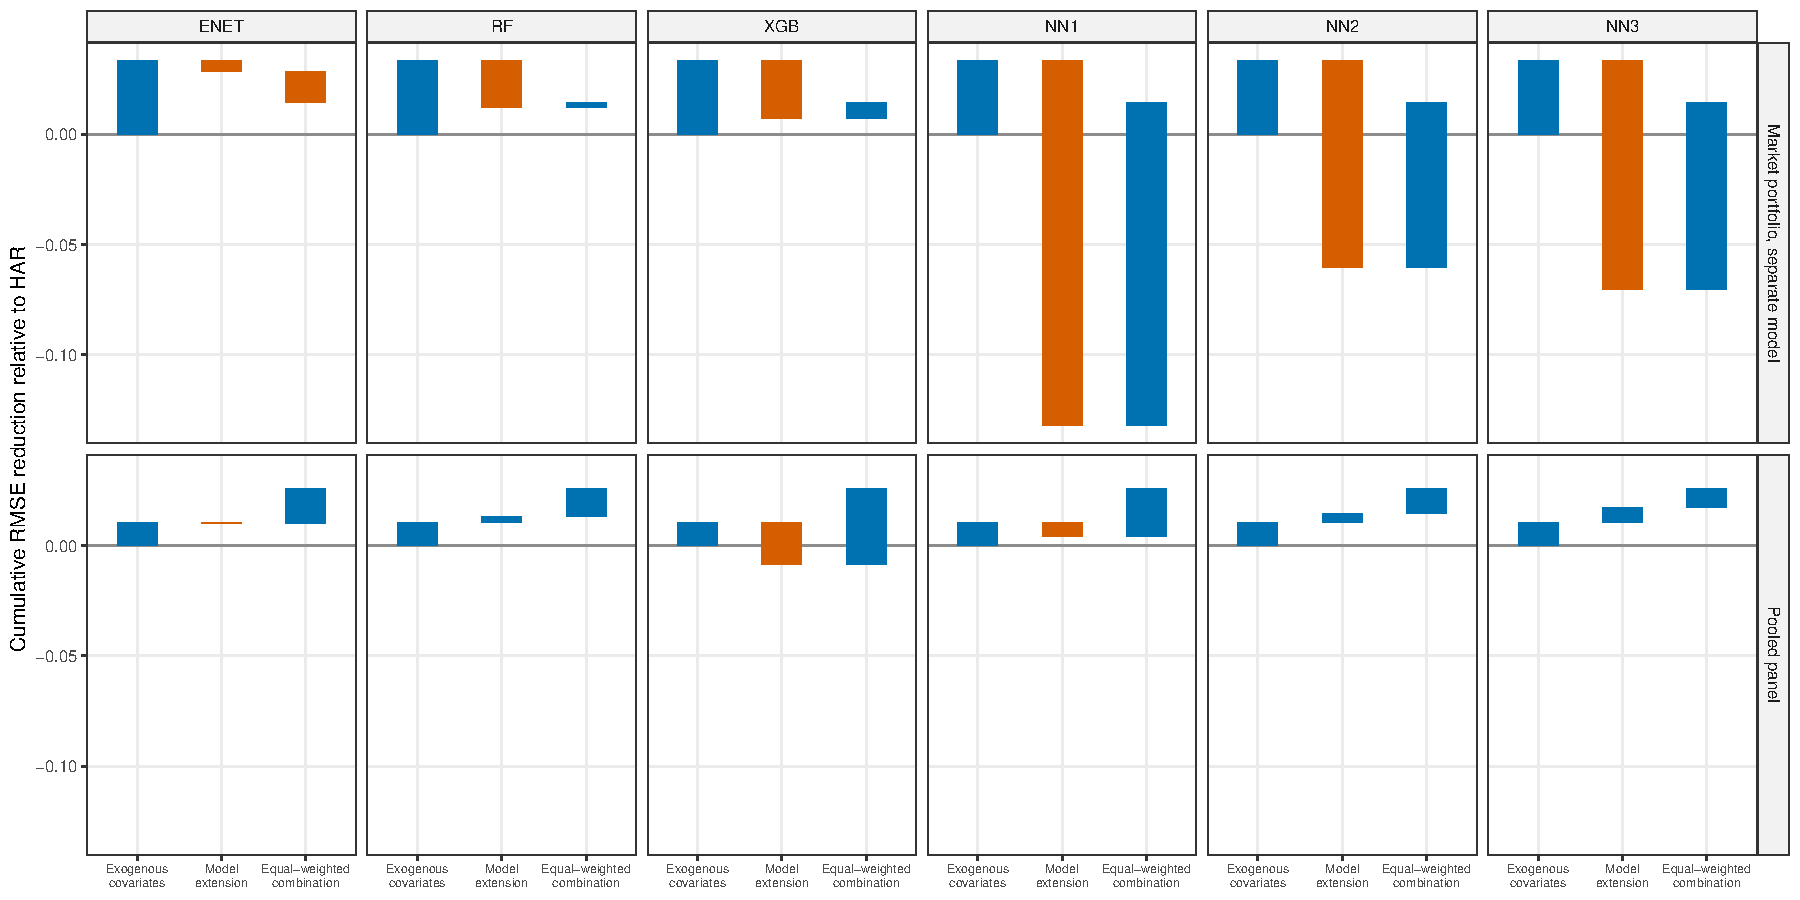
\includegraphics[width=\linewidth,height=0.70\textheight,keepaspectratio]{results_v3/1927/internet_appendix/sequential_waterfall.pdf}
\end{figure}
\begin{figure}[p]
\ContinuedFloat
\centering
\captionsetup{justification=raggedright,labelsep=none,singlelinecheck=false,labelformat=boldlabel}
\caption[]{\footnotesize \textbf{: Sequential changes in out-of-sample RMSE relative to HAR.} Each column considers one extension of HARX. The bars first add exogenous covariates, then the indicated model extension, and finally the equal-weighted forecast combination. Positive changes represent lower RMSE. These arithmetic comparisons do not identify causal contributions. Continued.}
\par\smallskip\textbf{Panel B. Short sample}\par\smallskip
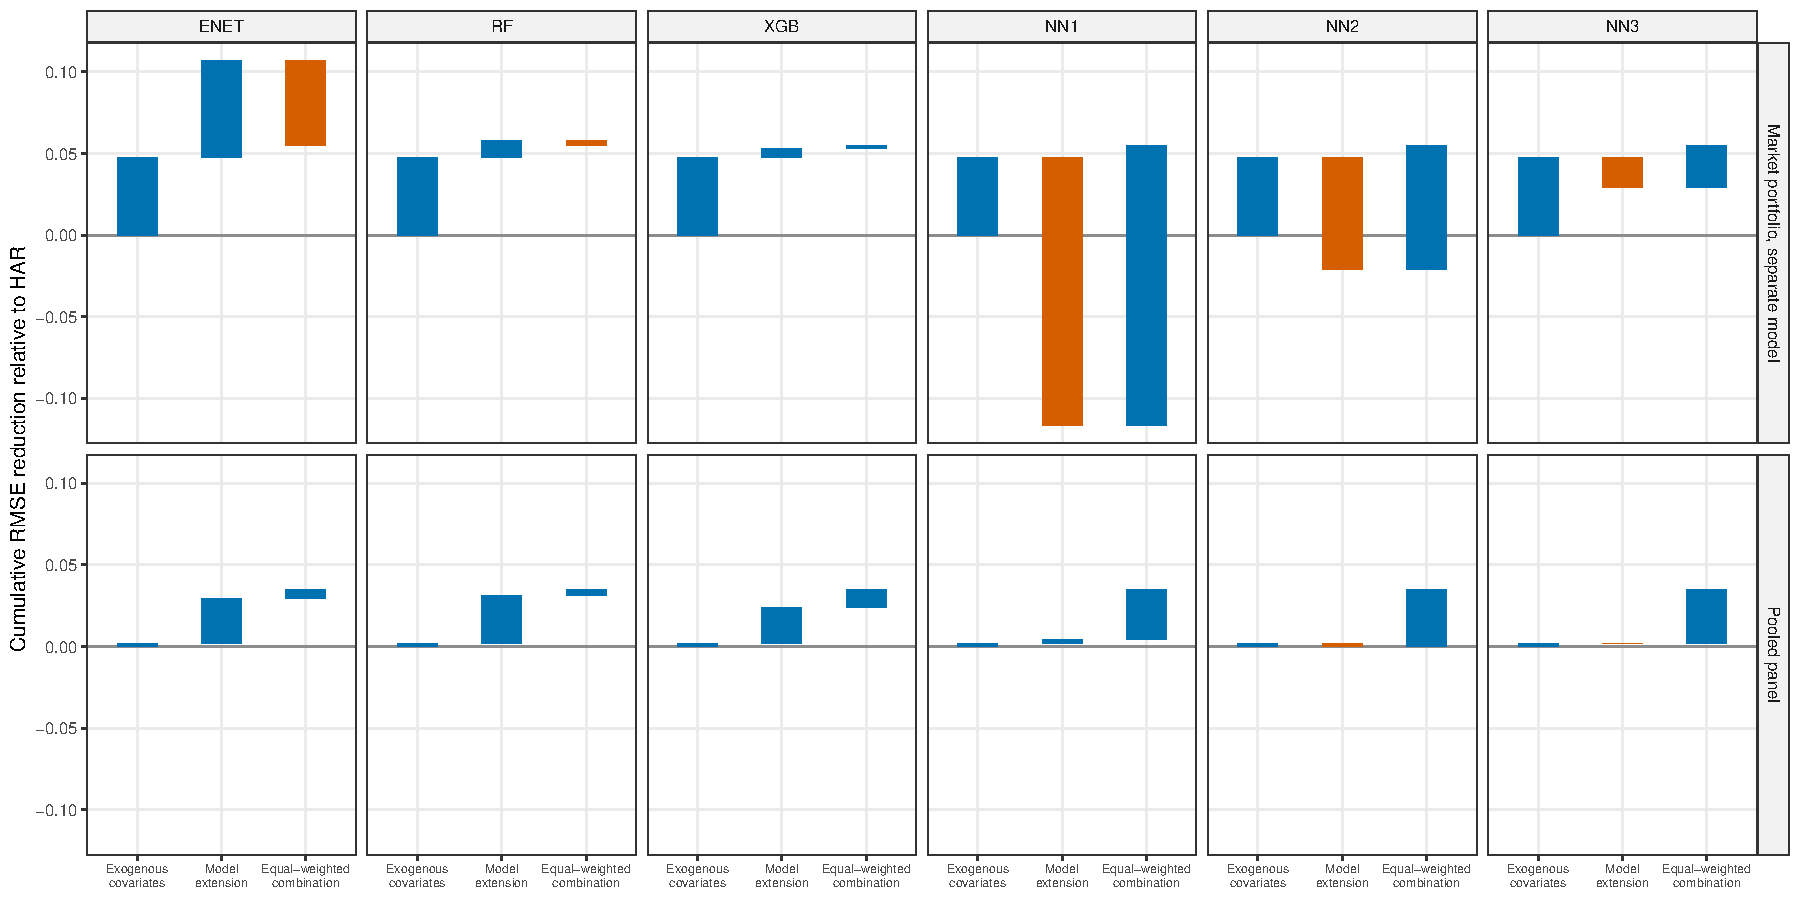
\includegraphics[width=\linewidth,height=0.70\textheight,keepaspectratio]{results_v3/1986/internet_appendix/sequential_waterfall.pdf}
\end{figure}
